\documentclass[a4paper,11pt]{article}
\usepackage[margin=1.5cm]{geometry}
\usepackage{amsmath}
\usepackage{amssymb}
\usepackage{color}
\usepackage{graphicx}
\usepackage{graphics}
\usepackage[margin=1.5cm]{geometry}
\usepackage{fancyhdr}
\usepackage{float}
\usepackage{wrapfig}
\usepackage{lscape}
\usepackage[font={small},labelfont=bf]{caption}
\usepackage{palatino}
\usepackage{mathpazo}

\bibliographystyle{unsrt}
%\linespread{1.2}

%%%%%%%
%Defines vectors universally, for ease of editing and consistency.
\newcommand{\vtr}[1] {\mathit{\underline{\boldsymbol{#1}}}}

%Draws a big red box containing the text as in \ALERT{<TEXT HERE>}. For labelling draft copies with important notes.
\def\ALERT#1{\begin{center}\colorbox{red}{\hbox{\textcolor{black}{\textbf{#1}}}}\end{center}}

%Roman-style subscript; removes math-mode font.
\def\s#1{_\textrm{#1} }

%The operators in integrals and derivatives.
\def\d{\operatorname{d}\!}

%The Euler e should be in Roman font.
\def\e{\textrm{e}}

%%%%%%%%%%%   some definitions used in latexing the CQMP:
% fractions that are of right size in set equations
\def\half{{\textstyle \frac{1}{2}}}
\def\quarter{{\textstyle \frac{1}{4}}}
\def\third{{\textstyle \frac{1}{3}}}
\def\eighth{{\textstyle \frac{1}{8}}}

% obtain a new line
\def\nl{\hfil\break}
\def\nll{\\ \\ \noindent}
%%%%%%%%%

%******************************* to optimise page usage
%\setlength{\textwidth}{6.3 in}

%\setlength{\oddsidemargin}{0.2 in}
%\setlength{\evensidemargin}{0.2 in}

%\setlength{\topmargin}{-.80 in}
%\setlength{\textheight}{9.9 in}
%*******************************

% to mark as a draft.  Comment both these lines out when complete.  The page number will return to the footer.
%\pagestyle{myheadings}
%\markright{\textcolor{red}{\textbf{DRAFT: \today}}}




\begin{document}
\setlength{\columnsep}{22pt}
%\vspace{-5cm}
%\maketitle
\textsc{\center \Large  Physical Concept: \textbf{Momentum and its conservation; collisions --- Part 1.}}
\vspace{0.4cm}

We briefly sketch definitions of momentum.  Understanding momentum further involves revising Newton's Laws and ideas about impulse, which are available at greater length at the concepts pages for Newton's Laws and for Impulse.  Collisions are a good area for illustration.  Part 2 for this concept addresses more powerful techniques for dealing with collisions, for instance as they arise in particle physics.

\section{Definition of momentum}
Momentum is mass $m$ times velocity $\vtr{v}$ for a particle: $\boxed{\vtr{p} = m \vtr{v}}$.\\
%\begin{equation*} \boxed{\vtr{p} = m \vtr{v}}
%\end{equation*}
It is a vector with units kg.m/sec.  Momentum can be carried by other entities, such as waves, but we just sketch mechanical momentum.

\section{Conservation of momentum}
The momentum is conserved in the absence of forces external to the system.  \\
This concept is one of the most important in physics consand follows from Newton's laws.  Newton's second law (N2L, ``force = mass times acceleration") can be written:
\begin{equation*} \vtr{f} = m \vtr{a} = m \d\vtr{v}/\d t = \d\vtr{p}/\d t .
\end{equation*}
N1L says that in the absence of forces, particles continue moving without further change of velocity.  Setting $\vtr{f}= 0$ in the above shows that then $\vtr{v}$ is unchanging, as is momentum $\vtr{p}$, that is momentum is conserved.\\
%\begin{wrapfigure}{r}{6cm}\vspace{-1cm}
%\center
%\includegraphics[width=0.3\textwidth]{collision.eps}
%\caption{The collision of two particles isolated from the rest of the world.}
%\label{fig:collision}
%\end{wrapfigure}
Consider a system consisting of two particles colliding head on, figure~\ref{fig:collision}. The box indicates the system is ``closed" --- there are forces within it (when the particles collide), but not on it from outside.

Momentum is always conserved, but energy can be converted to other forms (e.g. to heat) so collisions may or may not be elastic (that is conserving mechanical energy).  So one has:
\begin{equation*} \vtr{p}_1 +  \vtr{p}_2 = \vtr{p}_1'  + \vtr{p}_2'
\end{equation*}
where the prime $'$ indicates after the collision.\\
% \begin{wrapfigure}{r}{5cm}\vspace{-1cm}
%\center
%\includegraphics[width=0.25\textwidth]{inelastic.eps}
%\caption{The inelastic collision of two particles that stick together after colliding.}
%\label{fig:inelastic}
%\end{wrapfigure}
\begin{figure}[h!]% this one for two figures side by side
%\centering
\begin{minipage}{.45\textwidth}
  \centering
  \includegraphics[width=.7\linewidth]{collision.eps}
  \caption{The collision of two particles isolated from the rest of the world.}
  \label{fig:collision}
\end{minipage}\hfill
\begin{minipage}{.45\textwidth}
  \centering
  \includegraphics[width=.45\linewidth]{inelastic.eps}
  \caption{The inelastic collision of two particles that stick together after colliding.}
  \label{fig:inelastic}
\end{minipage}
\end{figure}

\nl
{\bf Levels 1--4.  Examples}
\nl
1.  Figure~\ref{fig:inelastic} shows two particles colliding and then sticking together.\\
If $m_1 = 1 \textrm{kg}$, $m_2 = 2\textrm{kg}$, $v_1 = 3 \textrm{m s}^{-1}$ and
$v_2 = 1\textrm{m s}^{-1}$, then the momentum is $1 \times 3 + 2 \times 1  = 5 \textrm{kg m s}^{-1}$.
It remains this value and hence after the collision one has $5 \textrm{kg m s}^{-1} = 3 \textrm{kg} \times v' \; \textrm{m s}^{-1}$.  Thus $ v' = 5/3 \; \textrm{m s}^{-1}$.
\nl
Calculate how much energy has been lost in the collision by calculating the total kinetic energy before and after.\\
Describe the collision (with sticking) in the case $m_1 = m_2 = 1\textrm{kg}$.\\

\vfill\break

\nl
2.  Consider two particles of equal mass, $m_1 = m_2 = m$ where $v_1 = v$ simply, and the other particle is initially at rest, $v_2=0$.  They collide elastically; see figure~\ref{fig:elastic}.  What are the final speeds $v_1'$ and $v_2'$?
%\begin{wrapfigure}{r}{5cm}
%\center
%\includegraphics[width=0.25\textwidth]{elastic.eps}
%\caption{An elastic collision of two equal particles, one being initially at rest.}
%\label{fig:elastic}
%\includegraphics[width=0.2\textwidth]{wall.eps}
%\caption{A particle colliding with a wall.  In the intermediate state it is instantaneously at rest and deformed.} \vspace{-1.0cm}
%\label{fig:wall}
%\end{wrapfigure}

\begin{figure}[h!]% this one for two figures side by side
%\centering
\begin{minipage}{.45\textwidth}
  \centering
  \includegraphics[width=.8\linewidth]{elastic.eps}
  \caption{An elastic collision of two equal particles, one being initially at rest.}
  \label{fig:elastic}
\end{minipage}\hfill
\begin{minipage}{.45\textwidth}
  \centering
  \includegraphics[width=.45\linewidth]{wall.eps}
  \caption{A particle colliding with a wall.  In the intermediate state it is instantaneously at rest and deformed.}
  \label{fig:wall}
\end{minipage}
\end{figure}

\nl Conserving momentum gives: $m v = m (v_1' + v_2')$ hence $v = v_1' + v_2'$.\\
Conserving energy gives: $\half m v^2 = \half m (v_1'^2 + v_2'^2)$.  Hence
$v^2 = v_1'^2 + v_2'^2$.
\nl
Put $v_1'  = v - v_2'$ from above into this energy relation:
\begin{equation*} v^2 = (v - v_2')^2 + v_2'^2  = v^2 - 2 v v_1' +v_1'^2 + v_1'^2\\
\rightarrow 2 v v_2' = 2 v_2'^2  \rightarrow v_2' = v .
\end{equation*}
Put this value of $v_2'$ into the momentum relation and find that $v_1' = 0$.
\nl
The first particle stops and the second continues with the velocity (and momentum) of the first --- like in Newton's cradle.

\nl
3.  A particle bouncing off a wall; figure~\ref{fig:wall}.\\

The incident particle has a force from the wall acting on it during the collision.  Momentum of the particle is not conserved. But \textit{the total momentum} of the particle plus the wall \textit{is conserved}.\\
  What is the change of momentum if the collision is elastic? (Remember momentum and its changes are vectors -- your answer requires a magnitude and a direction.)\\
 What is the momentum change if the collision is completely inelastic?


\section{Impulse}
Impulse is the change of momentum.  It is force times time, for a constant force acting.  The term is generally (but not always) used when momentum is transferred over a short time (e.g. during a collision).  It is described fully in the impulse concepts sheet.

\end{document}
